\chapter{Implementazione}\label{ch:implementation}
  In questo \nameCref{ch:implementation} sono esposti tutti i dettagli legati al processo di sviluppo e all'implementazione.
  In particolare, per quanto possibile verranno motivate le scelte tecnologiche che in fase di progettazione non erano state considerate rilevanti.
  Inoltre, verranno analizzati alcuni dettagli implementativi ritenuti importanti alla descrizione del funzionamento del progetto.

  \section{Tecnologie utilizzate}

  \subsection{Linguaggi di programmazione}
    Il sistema è stato realizzato in due differenti linguaggi. Di seguito sono espresse le motivazioni della scelta di ciascuno di essi.

    \subsubsection{Linguaggio per il backend: Kotlin}

      Per la realizzazione del backend, come è stato specificato nel~\Cref{ch:requirements}, era necessario l'impiego di un linguaggio in grado di eseguire su piattaforma JVM\@.
      Il framework scelto, Vert.x, è presentato come poliglotta (supporta Java, JavaScript, Groovy, Ruby, Ceylon, Scala e Kotlin) e non vincolava la scelta.

      Si è deciso di procedere con Kotlin per le seguenti motivazioni:

      \begin{description}
        \item[Brevità ed espressività]
          Kotlin si presenta come molto meno verboso di Java, supportando un maggior numero di costrutti che permettono di ridurre il codice ``\emph{boilerplate}''.

        \item[Sicurezza]
          Una delle funzionalità che è stata pubblicizzata maggiormente alla presentazione di Kotlin è la \emph{null-safety}.
          Kotlin permette di evitare le comuni eccezioni di tipo \texttt{NullPointerException} gestendo il valore \texttt{null} in modo maggiormente chiaro tramite notazione opzionale e controllo da parte del compilatore.

        \item[Interoperabilità]
          Kotlin nasce per essere affiancato a Java e sostituirlo gradualmente.
          Risulta dunque intercompatibile con quasi qualsiasi piattaforma o libreria sia pensata per Java, non limitando eventualmente l'affiancamento futuro ad un altro linguaggio.

          Inoltre, il compilatore di Kotlin supporta diversi altri target, come browser, piattaforme mobile e binario nativo X86 e ARM, lasciando dunque aperte ulteriori possibilità di espansione future.

        \item[Approccio funzionale]
          Kotlin è un linguaggio orientato agli oggetti, ma supporta molti costrutti tipici della programmazione funzionale, come espressioni \emph{lambda}, \emph{function types} e le funzioni di ordine superiore.

        % \item[Performance]
          % Kotlin  pone  alcuni  miglioramenti  prestazionali nelle funzioni di ordine superiore e lambda, dimostrandosi più ottimizzato e veloce nei confronti di Java

        \item[Pragmatismo]
          Kotlin presenta, secondo la documentazione, l'intento di essere ``pragmatico'', ossia focalizzato sull'esperienza d'uso dello sviluppatore.
          Esso offre una buona integrazione con gli strumenti esistenti, sia per la costruzione (come Gradle e Maven) che per lo sviluppo (come Eclipse, Visual Studio e gli IDE di JetBrains).
      \end{description}

      Vert.x offre inoltre una estensione della propria libreria \emph{core} per sfruttare al meglio la sintassi di Kotlin.

    \subsubsection{Linguaggio per il frontend: TypeScript}\label{subsub:ts}
      Per la realizzazione del frontend era necessario l'impiego di un linguaggio in grado di eseguire su browser, quindi che fornisse come target di compilazione JavaScript o WebAssembly.
      A differenza del backend, il framework scelto, React, vincolava la scelta a un numero limitato di linguaggi in grado di generare codice JS\@.
      In particolare, sono stati presi in considerazione i quattro linguaggi introdotti nella~\Cref{sec:lang}, ma si è preferito impiegare TypeScript per i seguenti motivi:

      \begin{description}
        \item[Supporto ufficiale]
          Per quanto React venga presentato anche nella documentazione ufficiale~\cite{react-docs} come non strettamente dipendente dal linguaggio, il supporto disponibile per ciascuno di questi può essere differente.
          In particolare, Facebook, dichiara il supporto diretto solo per JavaScript e TypeScript;
          linguaggi come Kotlin, Scala, Reason e F\# sono dichiaratamente compatibili, ma la loro integrazione non è una priorità per la società.

          Kotlin (attraverso JetBrains) e Scala (attraverso il progetto Scala.js) offrono un supporto comunitario sufficiente, ma comunque non comparabile a quello offerto da Facebook e Microsoft.\unsure{Dovrei citare statistici da GitHub per sostenere questa posizione?}

        \item[Type Checking]
          JavaScript supporta unicamente la tipizzazione dinamica.
          Se questo aspetto da un lato aggiunge flessibilità al linguaggio, dall'altro aumenta la possibilità di bug e situazioni non previste.
          TypeScript offre un sistema di tipi completo e flessibile, che permette di definire una struttura chiara e flessibile, rendendo il processo di sviluppo più sicuro.

          Facebook supporta ufficialmente Flow e la libreria \texttt{prop-types} come alternativa all'utilizzo di un diverso linguaggio.
          Flow non offre però la medesima espressività di TypeScript e non può vantare un supporto altrettanto vasto da parte della comunità per la tipizzazione delle librerie JavaScript.
          La libreria \texttt{prop-types} invece offre un controllo dei tipi unicamente a tempo di esecuzione, richiedendo la definizione del tipo atteso manualmente.
          Questo non permette di adottare un approccio ``\emph{fail-fast}'' come quello vantato da TypeScript.

        \item[Integrazione con gli IDE]
          La possibilità di avere informazione sui tipi a livello di compilatore permettono a IDE come Visual Studio Code e WebStorm di essere molto più precisi ad evidenziare codice errato rispetto all'approccio basato su commenti di JavaScript.

        \item[Estensione della sintassi JSX e TSX]
          Una delle maggiori particolarità del framework React è la sintassi \emph{JSX}\@.
          L'acronimo sta per \emph{\emph{J}ava\emph{S}cript e\emph{X}tension} e identifica un particolare zucchero sintattico non presente in JavaScript ``standard''.
          Esso permette la definizione di ``\texttt{element}'', ossia di componenti direttamente rappresentabili, attraverso una sintassi dichiarativa di markup che ricorda HTML\@. \unsure{Dovrei inserire uno snippet di confronto?}

          Essendo in React la logica rappresentativa strettamente legata agli elementi non grafici del componente, essere in grado di distinguere in modo chiaro i \emph{concetti}\improvement{Non sono sicuro di aver espresso correttamente in italiano ``separation of concerns'', che sarebbe da traduzione separazione di interessi}
          all'interno dello stesso componente e file senza doversi affidare a markup esterno è un vantaggio notevole.

          TypeScript supporta questa estensione della sintassi, denominandola \emph{TSX}.

      \end{description}

      L'unica alternativa presa in considerazione al posto di TypeScript era Kotlin.
      L'impiego di Kotlin per tutta l'applicazione sarebbe stato infatti molto interessante per utilizzare un unico linguaggio in tutto il sistema, migliorando l'integrazione e il supporto a dipendenze condivise.

      Purtroppo, per quanto JetBrains supporti ufficialmente React per Kotlin/JS, l'integrazione all'inizio dei lavori di questa tesi era ancora troppo instabile per un uso reale.
      Si sono riscontrati problemi con lo strumento di generazione dei \emph{wrapper} per i tipi\unsure{Dovrei citare la issue GitHub che avevamo creato?} e l'output del compilatore genera codice JS datato e pesante.
      Fintanto che la versione 1.4 di Kotlin non sarà rilasciata in pianta stabile, si ritiene che il linguaggio non sia ancora pronto per un uso frontend su browser.

  \subsection{Strumenti per lo sviluppo e il controllo del software}\label{subec:quality}
    Per gestire le dipendenze in sistemi moderni, l'uso di applicazioni per la \emph{build-automation} dotati di risoluzione delle dipendenze è l'approccio più comune.

    L'utilizzo di strumenti che controllino la qualità del codice e diano la possibilità di testarlo in modo immediato è invece fondamentale per la realizzazione di un sistema complesso.
    Essi permettono infatti di revisionare il codice in modo sistematico, così da evitare errori che a volte possono verificarsi, senza bisogno che il programma venga realmente eseguito:
    analizzano il codice sorgente per individuare potenziali bug e spesso indicano possibili miglioramenti e ottimizzazioni.
    % Spesso tali strumenti vengono integrati nel processo di costruzione del codice.

    Essendo le due componenti basate su ecosistemi completamente diversi, verranno trattate separatamente.

    \subsubsection{Backend}

      Il progetto di backend utilizza Gradle per la risoluzione delle dipendenze, la costruzione del software e la verifica della qualità.
      Gradle è un sistema per l'automazione dello sviluppo, nato per includere tutte le caratteristiche provenienti da Apache Ant, Maven e Ivy attraverso la definizione di \engEmph{buildscript} in Groovy e, più recentemente, in Kotlin.
      Pensato per i linguaggi che compilano per JVM, questo sistema permette di scaricare le dipendenze da diversi repository Maven durante la fase di compilazione.
      Nello script di costruzione sono stati utilizzati i seguenti plugin:

      \begin{description}
        \item[Gradle Shadow]
          Il plugin, sviluppato da John Engelman, permette la generazione di ``shadow jar'', ossia pacchetti jar contenenti anche tutte le dipendenze oltre al codice compilato.

        \item[Vert.x Gradle Plugin]
          Il plugin, sviluppato da Julien Ponge e adottato semi-ufficialmente dai manutentori del progetto Vert.x, fornisce una configurazione del progetto ottimizzata per progetti Vert.x.
          Rende possibile il lancio dei verticle in modo indipendente e con la ricompilazione automatica, molto comodo in sede di sviluppo e debug.

        \item[Kotlin]
          Il plugin, realizzato in modo ufficiale da JetBrains, configura Gradle per la compilazione di codice Kotlin e la configurazione delle opzioni per la generazione del bytecode.

          Per motivi di compatibilità con il simulatore Alchemist, è stata scelta come versione target del bytecode Java 11.

        \item[Ktlint Gradle]
          Il plugin, realizzato da Jonathan Leitschuh, è un wrapper dello strumento di analisi statica di codice Kotlin \emph{ktlint}, realizzato da Pinterest.
          Si è scelto di utilizzare ktlint anziché \emph{detekt}, altro strumento simile, in quanto non richiede una configurazione personalizzata, bensì impone un insieme standard di regole, comunemente studiate e accettate dalla community.

        \item[refreshVersions]\unsure{Qui la minuscola è \emph{voluta}, in quanto il plugin non ha un nome formale. Dovrei metterlo comunque maiuscolo come gli altri?}
          Il plugin, sviluppato da Jean-Michel Fayard, permette una migliore gestione delle dipendenze automatizzandone gli aggiornamenti.

        \item[JUnit]
          JUnit è uno dei più noti framework di unit testing per Java e linguaggi derivati.
          Il plugin, integrato ufficialmente in Gradle, permette l'esecuzione di test automatizzati con tale framework.

          In questo progetto è stata utilizzata la versione 5 di JUnit, utilizzando il motore di esecuzione \emph{jupiter}.
        \item[JaCoCo]
          JaCoCo è uno strumento per la misura della copertura del codice da parte dei test realizzati.
          Si integra con JUnit ed è pensato per Java e linguaggi derivati.
          Il plugin, integrato ufficialmente in Gradle, offre una dettagliata configurazione e permette la generazione di report in diversi formati.
      \end{description}

      Per lo sviluppo del codice è stato utilizzato l'ambiente di sviluppo integrato \emph{JetBrains Intellij IDEA} in versione \emph{Ultimate 2019.3.3}.
      Si è scelto questo rispetto ad altri IDE (come ad esempio Eclipse) in quanto in grado di offrire un'integrazione migliore con Gradle e Kotlin.

    \subsubsection{Frontend}

      Il progetto frontend è un modulo Node.js generato tramite lo strumento ufficiale \texttt{create-react-app} fornito da Facebook.
      Si seguito vengono riportate tutte le tecnologie utilizzate durante lo sviluppo:

      \begin{description}
        \item[Yarn]
          Come \emph{package manager} per la gestione delle dipendenze è stato scelto yarn anziché NPM\@.
          Esso, oltre a essere la scelta consigliata da React, presenta alcuni vantaggi rispetto alla controparte:
          \begin{itemize}
            \item La cartella delle dipendenze risulta generalmente più compatta in quanto utilizza collegamenti simbolici per le dipendenze condivise dai moduli JS risolti.
            \item La velocità di risoluzione delle dipendenze è generalmente più elevata, in quanto sfrutta una strategia di cache più efficiente.
          \end{itemize}

        \item[react-scripts]
          Lo strumento \texttt{create-react-app} astrae la complessità di configurazione di un progetto attraverso l'utilizzo di \texttt{react-scripts}.
          Essi incapsulano strumenti quali WebPack, Babel, ESLint e Jest, mettendo a disposizione semplici script che si appoggiano alle configurazioni ufficiali di riferimento per:
          \begin{inparaitem}
            \item compilazione,
            \item esecuzione,
            \item verifica
          \end{inparaitem}
          del codice realizzato.

        \item[ESLint \& stile Airbnb]
          ESLint è uno strumento estendibile per l'analisi statica del codice, che supporta nativamente JavaScript e TypeScript.
          Il pacchetto \texttt{react-scripts} fornisce una configurazione minimale, ma consiglia di adottare uno stile (insieme di regole) tra quelli più famosi;
          è stato scelto quello fornito da Airbnb. % , in quanto uno dei più popolari.

        \item[Jest]
          Jest è un framework di test per JavaScript sviluppato da Facebook che fornisce tutti gli strumenti per la scrittura e l'esecuzione dei test e per la raccolta della loro copertura sul codice.
      \end{description}

      Per lo sviluppo del codice è stato utilizzato l'ambiente di sviluppo integrato \emph{JetBrains WebStorm} in versione \emph{2019.3.3}.

  \subsection{Controllo di versione e CI/CD}
    Il controllo di versione utilizzato per questo progetto è affidato al DVCS (\emph{\emph{D}istributed \emph{V}ersion \emph{C}ontrol \emph{S}ystem}) Git, utilizzato con flusso di lavoro di tipo \emph{Git flow}.

    % Il codice è disponibile su GitHub nei repository seguenti:
    % \begin{itemize}
    %     \item \url{https://github.com/NiccoMlt/Protelis-Web} per il backend;
    %     \item \url{https://github.com/NiccoMlt/protelis-web-frontend} per il frontend.
    % \end{itemize}

    Il codice è disponibile su GitHub nei repository GitHub Protelis-Web\footnote{\url{https://github.com/NiccoMlt/Protelis-Web}}\improvement{Dovrei creare un DOI con Zotero?}
    e protelis-web-frontend\footnote{\url{https://github.com/NiccoMlt/protelis-web-frontend}}.
    % Si è preferito utilizzare due depositi separati anziché raggruppare in ciò che viene generalmente definito \emph{monorepo} poiché le differenti ...

    Attraverso GitHub sono allacciate ai repository le soluzioni di \emph{continuous integration} (CI):

    \begin{description}
      \item[Travis CI]
        Travis CI è un sistema di integrazione continua distribuito, utilizzato per la compilazione e il test di progetti caricati su repository GitHub.
        Ad ogni operazione di push sul repository, il codice viene testato su tutte le maggiori piattaforme (Linux, Windows, MacOS) e le differenti versioni degli SDK (NodeJS LTS, AdoptOpenJDK con OpenJDK HotSpot e AdoptOpenJDK con Eclipse OpenJ9).
        Viene inoltre fatto un controllo sulla qualità del codice.

      \item[Codecov]
        Tramite Codecov vengono raccolti i report di copertura del codice generati da JaCoCo e Jest, permettendo la visualizzazione online di grafici di dettaglio.
        Al termine di ogni esecuzione di una \emph{pipeline} in Travis CI, i report sulla piattaforma di riferimento vengono pubblicati qui.

      \item[Codacy]
        Codacy è uno strumento online per l'automazione della \emph{code review} che aggrega diversi strumenti di analisi del codice per numerosi linguaggi, generando report dettagliati.
        Ad ogni operazione di push sul repository, il codice viene verificato.
    \end{description}

  \subsection{Deployment}
    Vert.x non si basa su \emph{servlet} e può essere eseguito su qualsiasi piattaforma permetta il lancio di un jar.

    Per motivi di test, il server è in esecuzione su due differenti piattaforme:

    \begin{itemize}
      \item
        Al termine della pipeline di Travis CI per il branch principale, l'eseguibile viene automaticamente caricato e lanciato su Heroku.

        \emph{Heroku} è un servizio online di tipo PaaS (\emph{\emph{P}latform as a \emph{S}ervice}) di proprietà di SalesForce e compatibile con diversi linguaggi.
        Informazioni sulla VM utilizzata non sono disponibili.
      \item
        Per performance migliori, viene utilizzato anche un server fornito dall'Università di Bologna.
        Su di esso viene effettuato il deploy tramite SSH avvalendosi del \texttt{docker-engine} in esecuzione all'interno di Linux.

        \emph{Docker} è uno strumento per la virtualizzazione a livello di sistema operativo (\emph{container}) molto utilizzato per la pacchettizzazione delle applicazioni.
        Il Dockerfile per la costruzione dell'immagine utilizzata, basato su AdoptOpenJDK con Eclipse OpenJ9, è allegato a questo documento in~\Cref{app:docker}.
    \end{itemize}

    Il client React è compilato come un bundle JavaScript importato da una pagina HTML\@.
    Esso non viene servito dal server Vert.x, bensì dalla piattaforma Zeit Now, che ne esegue il \emph{continuous deployment} direttamente da GitHub.

    % Per quanto riguarda il \emph{continuous deployment} (CD), sarà trattato nel dettaglio nella sottosezione successiva.

      % \subsection{Librerie esterne}
  % \subsection{Strumenti di sviluppo}
  %   In questa sezione verranno presentati tutti gli strumenti utilizzati per sviluppare il codice del sistema,
  %   descrivendone la loro utilità e il loro impiego.

  %   \subsubsection{Ambiente di sviluppo}
  %     Un IDE, o \emph{Integrated Development Environment} è un software che aiuta i programmatori nello sviluppo del codice sorgente di un software.\unsure{Non sono sicuro che questa parte sia necessaria}
  %     Esso mette a disposizione tutta una serie di strumenti e funzionalità utili per lo sviluppo e il debugging.
  %     Solitamente uno strumento di questo tipo mette a disposizione un editor di testo, un compilatore o un interprete (o entrambi) e un debugger.

  %     Per lo sviluppo di questo sistema sono stati utilizzati due IDE forniti da JetBrains: Intellij IDEA e WebStorm.
  %     In particolare,


  \section{Dettagli implementativi: Frontend}

    Per l'implementazione dei componenti di base del frontend, si è fatto largo uso della libreria Material-UI\@.
    Essa mette a disposizione una grande quantità di componenti React di base (come elementi per il layout e elementi di controllo) aderenti al design Material scelto in fase di progettazione.
    Inoltre, tramite la libreria è stato possibile definire un tema specifico per il progetto Protelis on Web nelle due varianti chiara e scura, caricate a seconda delle preferenze del browser dell'utente.

    \begin{figure}[htbp]
      \centering
      \includegraphics[width=\textwidth]{res/screenshot/Screenshot_2020-03-02 Protelis on the Web(6).png} % ChkTeX 8, ChkTeX 36
      \caption{Screenshot della schermata intera durante l'esecuzione}%
      \label{fig:screenshot:all}
    \end{figure}

    La struttura del frontend, visibile in~\Cref{fig:screenshot:all}, è composta da tre elementi principali:

    \begin{itemize}
      \item
        la \texttt{AppBar} superiore, nella quale è posizionato il selettore con il quale è possibile indicare quale server di backend utilizzare.
      \item
        la \texttt{Card} di sinistra ospita tutti i controlli principali.
        In essa è presente un editor realizzato con l'ausilio della libreria Monaco Editor, realizzata da Microsoft e utilizzata, ad esempio, per Visual Studio Code;
        Essa supporta buona parte dei plugin disponibili per tale IDE e lascia spazio, in futuro, all'integrazione di \emph{language server} dedicati all'autocompletamento.

        Sotto l'editor sono presenti i bottoni dedicati al salvataggio del codice e all'avvio dell'esecuzione.
      \item
        la \texttt{Card} di destra ospita invece principalmente un canvas, realizzato tramite la libreria Konva.
        Essa permette di realizzare canvas performanti modellando ciascuna operazione di disegno come componenti React.

        È risultato dunque semplice delegare le operazioni di disegno al motore di React, attraverso un'operazione di binding dei componenti di Konva con lo store di Redux.
    \end{itemize}

    \unsure[inline]{Potrebbe essere utile documentare la realizzazione del \strong{middleware} per l'\strong{EventBus}?}

    \improvement[inline]{Possono essere interessanti altri dettagli?}

  \section{Dettagli implementativi: Backend}

    Come progettato nella~\Cref{sec:arch:server}, il server è stato realizzato con due verticle di Vert.x che modellano la logica applicativa e uno dedicato all'avvio del sistema.
    Tali verticle comunicano tra loro e con l'esterno tramite EventBus.

    L'EventBus viene esposto verso l'esterno tramite la libreria ufficiale di Vert.x per la realizzazione di bridge con SockJS\@.
    In particolare, la classe \texttt{BridgeVerticle} si occupa di costruire un router HTTP e HTTPS sul quale viene montato il bridge.

    La gestione della simulazione avviene, come detto, appoggiandosi ad Alchemist (il diagramma UML in~\Cref{fig:server:uml} mostra le principali classi coinvolte).

    \begin{figure}[htbp]
      \centering
      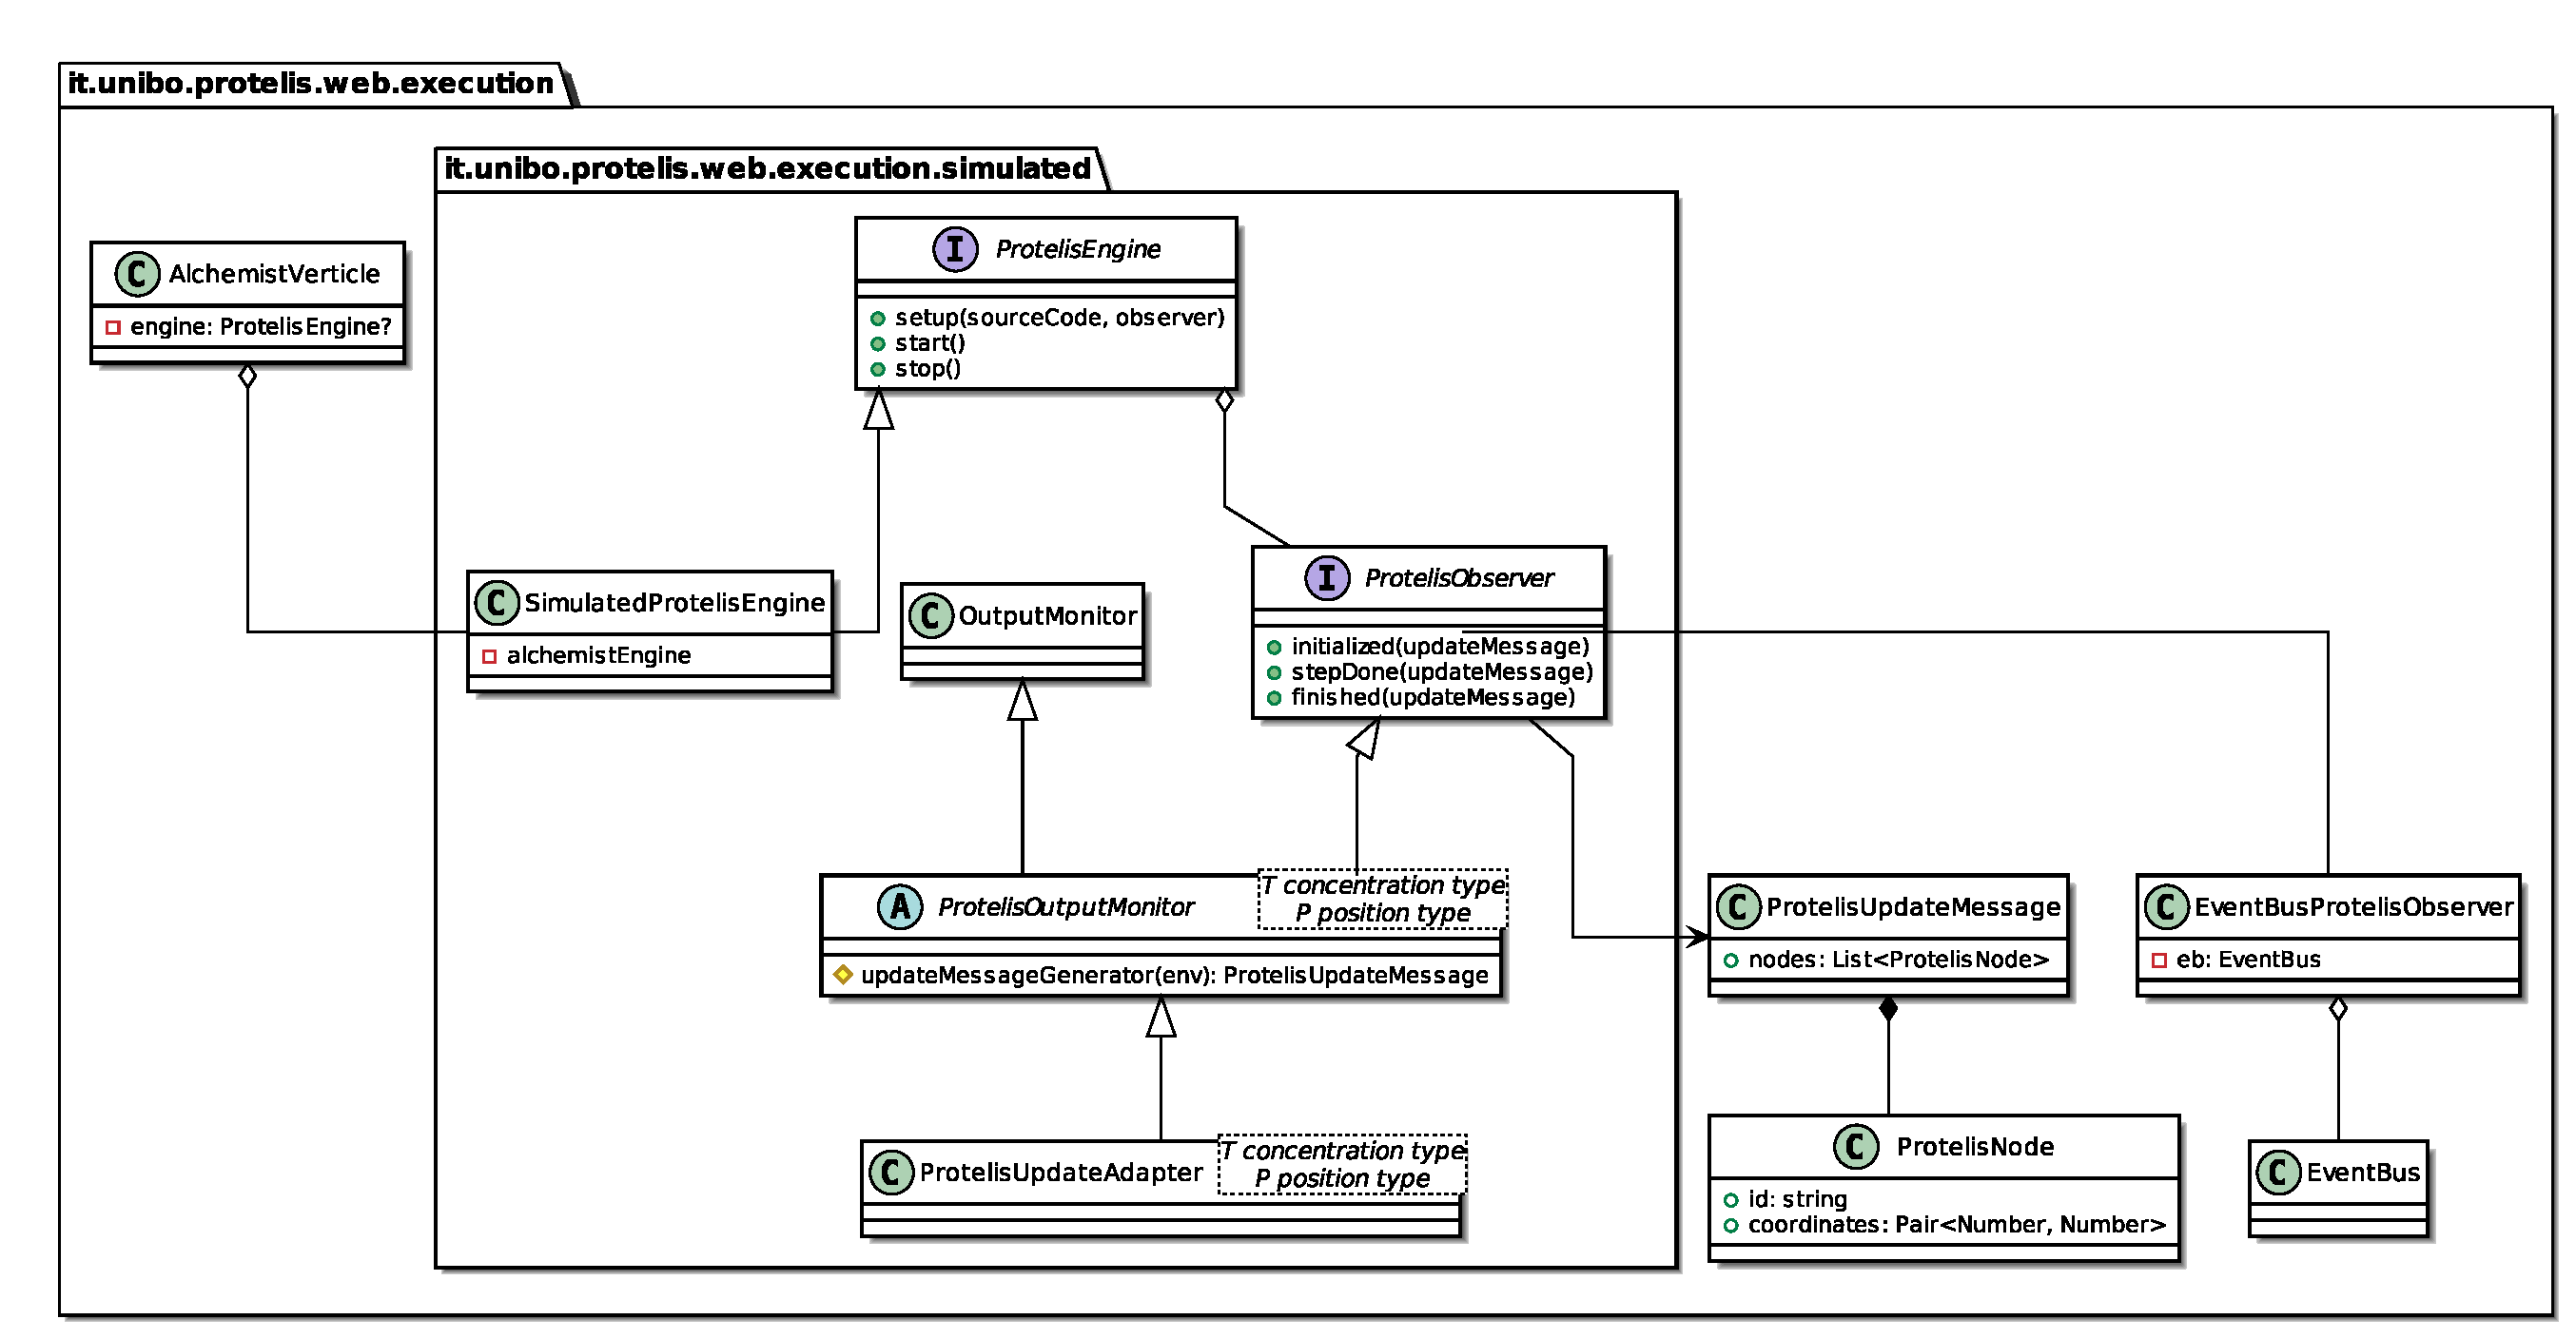
\includegraphics[width=\textwidth]{res/uml/engine-simple.eps}
      \caption{Rappresentazione UML delle classi coinvolte nella simulazione}%
      \label{fig:server:uml}
    \end{figure}

    Come è possibile vedere, Alchemist non viene utilizzato direttamente, bensì incapsulato all'interno di un \texttt{SimulatedProtelisEngine}.
    Tale classe implementa l'interfaccia \texttt{ProtelisEngine}, che astrae il concetto di esecutore per codice Protelis;
    in questo modo, il sistema non è vincolato all'implementazione simulata, né essa è legata strettamente ad Alchemist.

    Anche l'astrazione di Alchemist per l'osservazione del motore di esecuzione è stata incapsulata, definendo una classe di \emph{boundary}, \texttt{ProtelisOutputMonitor}, che agisce da adattatore.

    \improvement[inline]{Possono essere interessanti altri dettagli?}
